% !Mode:: "TeX:UTF-8"
\documentclass[12pt,a4paper]{article}

%%%%%%%%------------------------------------------------------------------------
%%%% 日常所用宏包

%% 控制页边距
% 如果是beamer文档类, 则不用geometry
\makeatletter
\@ifclassloaded{beamer}{}{\usepackage[top=2.5cm, bottom=2.5cm, left=2.5cm, right=2.5cm]{geometry}}
\makeatother

%% 控制项目列表
\usepackage{enumerate}

%% 多栏显示
\usepackage{multicol}

%% 算法环境
\usepackage{algorithm}  
\usepackage{algorithmic} 
\usepackage{float} 

%% 网址引用
\usepackage{url}

%% 控制矩阵行距
\renewcommand\arraystretch{1.4}

%% hyperref宏包,生成可定位点击的超链接,并且会生成pdf书签
\makeatletter
\@ifclassloaded{beamer}{
\usepackage{hyperref}
\usepackage{ragged2e} % 对齐
}{
\usepackage[%
    pdfstartview=FitH,%
    CJKbookmarks=true,%
    bookmarks=true,%
    bookmarksnumbered=true,%
    bookmarksopen=true,%
    colorlinks=true,%
    citecolor=blue,%
    linkcolor=blue,%
    anchorcolor=green,%
    urlcolor=blue%
]{hyperref}
}
\makeatother



\makeatletter % 如果是 beamer 不需要下面两个包
\@ifclassloaded{beamer}{
\mode<presentation>
{
} 
}{
%% 控制标题
\usepackage{titlesec}
%% 控制目录
\usepackage{titletoc}
}
\makeatother

%% 控制表格样式
\usepackage{booktabs}

%% 控制字体大小
\usepackage{type1cm}

%% 首行缩进,用\noindent取消某段缩进
\usepackage{indentfirst}

%% 支持彩色文本、底色、文本框等
\usepackage{color,xcolor}

%% AMS LaTeX宏包: http://zzg34b.w3.c361.com/package/maths.htm#amssymb
\usepackage{amsmath,amssymb}
%% 多个图形并排
\usepackage{subfig}
%%%% 基本插图方法
%% 图形宏包
\usepackage{graphicx}
\newcommand{\red}[1]{\textcolor{red}{#1}}
\newcommand{\blue}[1]{\structure{#1}}
\newcommand{\brown}[1]{\textcolor{brown}{#1}}
\newcommand{\green}[1]{\textcolor{green}{#1}}


%%%% 基本插图方法结束

%%%% pgf/tikz绘图宏包设置
\usepackage{pgf,tikz}
\usetikzlibrary{shapes,automata,snakes,backgrounds,arrows}
\usetikzlibrary{mindmap}
%% 可以直接在latex文档中使用graphviz/dot语言,
%% 也可以用dot2tex工具将dot文件转换成tex文件再include进来
%% \usepackage[shell,pgf,outputdir={docgraphs/}]{dot2texi}
%%%% pgf/tikz设置结束


\makeatletter % 如果是 beamer 不需要下面两个包
\@ifclassloaded{beamer}{

}{
%%%% fancyhdr设置页眉页脚
%% 页眉页脚宏包
\usepackage{fancyhdr}
%% 页眉页脚风格
\pagestyle{plain}
}

%% 有时会出现\headheight too small的warning
\setlength{\headheight}{15pt}

%% 清空当前页眉页脚的默认设置
%\fancyhf{}
%%%% fancyhdr设置结束


\makeatletter % 对 beamer 要重新设置
\@ifclassloaded{beamer}{

}{
%%%% 设置listings宏包用来粘贴源代码
%% 方便粘贴源代码,部分代码高亮功能
\usepackage{listings}

%% 设置listings宏包的一些全局样式
%% 参考http://hi.baidu.com/shawpinlee/blog/item/9ec431cbae28e41cbe09e6e4.html
\lstset{
showstringspaces=false,              %% 设定是否显示代码之间的空格符号
numbers=left,                        %% 在左边显示行号
numberstyle=\tiny,                   %% 设定行号字体的大小
basicstyle=\footnotesize,                    %% 设定字体大小\tiny, \small, \Large等等
keywordstyle=\color{blue!70}, commentstyle=\color{red!50!green!50!blue!50},
                                     %% 关键字高亮
frame=shadowbox,                     %% 给代码加框
rulesepcolor=\color{red!20!green!20!blue!20},
escapechar=`,                        %% 中文逃逸字符,用于中英混排
xleftmargin=2em,xrightmargin=2em, aboveskip=1em,
breaklines,                          %% 这条命令可以让LaTeX自动将长的代码行换行排版
extendedchars=false                  %% 这一条命令可以解决代码跨页时,章节标题,页眉等汉字不显示的问题
}}
\makeatother
%%%% listings宏包设置结束


%%%% 附录设置
\makeatletter % 对 beamer 要重新设置
\@ifclassloaded{beamer}{

}{
\usepackage[title,titletoc,header]{appendix}
}
\makeatother
%%%% 附录设置结束


%%%% 日常宏包设置结束
%%%%%%%%------------------------------------------------------------------------


%%%%%%%%------------------------------------------------------------------------
%%%% 英文字体设置结束
%% 这里可以加入自己的英文字体设置
%%%%%%%%------------------------------------------------------------------------

%%%%%%%%------------------------------------------------------------------------
%%%% 设置常用字体字号,与MS Word相对应

%% 一号, 1.4倍行距
\newcommand{\yihao}{\fontsize{26pt}{36pt}\selectfont}
%% 二号, 1.25倍行距
\newcommand{\erhao}{\fontsize{22pt}{28pt}\selectfont}
%% 小二, 单倍行距
\newcommand{\xiaoer}{\fontsize{18pt}{18pt}\selectfont}
%% 三号, 1.5倍行距
\newcommand{\sanhao}{\fontsize{16pt}{24pt}\selectfont}
%% 小三, 1.5倍行距
\newcommand{\xiaosan}{\fontsize{15pt}{22pt}\selectfont}
%% 四号, 1.5倍行距
\newcommand{\sihao}{\fontsize{14pt}{21pt}\selectfont}
%% 半四, 1.5倍行距
\newcommand{\bansi}{\fontsize{13pt}{19.5pt}\selectfont}
%% 小四, 1.5倍行距
\newcommand{\xiaosi}{\fontsize{12pt}{18pt}\selectfont}
%% 大五, 单倍行距
\newcommand{\dawu}{\fontsize{11pt}{11pt}\selectfont}
%% 五号, 单倍行距
\newcommand{\wuhao}{\fontsize{10.5pt}{10.5pt}\selectfont}
%%%%%%%%------------------------------------------------------------------------


%% 设定段间距
\setlength{\parskip}{0.5\baselineskip}

%% 设定行距
\linespread{1}


%% 设定正文字体大小
% \renewcommand{\normalsize}{\sihao}

%制作水印
\RequirePackage{draftcopy}
\draftcopyName{XTUMESH}{100}
\draftcopySetGrey{0.90}
\draftcopyPageTransform{40 rotate}
\draftcopyPageX{350}
\draftcopyPageY{80}

%%%% 个性设置结束
%%%%%%%%------------------------------------------------------------------------


%%%%%%%%------------------------------------------------------------------------
%%%% bibtex设置

%% 设定参考文献显示风格
% 下面是几种常见的样式
% * plain: 按字母的顺序排列,比较次序为作者、年度和标题
% * unsrt: 样式同plain,只是按照引用的先后排序
% * alpha: 用作者名首字母+年份后两位作标号,以字母顺序排序
% * abbrv: 类似plain,将月份全拼改为缩写,更显紧凑
% * apalike: 美国心理学学会期刊样式, 引用样式 [Tailper and Zang, 2006]

\makeatletter
\@ifclassloaded{beamer}{
\bibliographystyle{apalike}
}{
\bibliographystyle{unsrt}
}
\makeatother


%%%% bibtex设置结束
%%%%%%%%------------------------------------------------------------------------

%%%%%%%%------------------------------------------------------------------------
%%%% xeCJK相关宏包

\usepackage{xltxtra,fontspec,xunicode}
\usepackage[slantfont, boldfont]{xeCJK} 
\usepackage{bm}

\setlength{\parindent}{2em}%中文缩进两个汉字位

%% 针对中文进行断行
\XeTeXlinebreaklocale "zh"             

%% 给予TeX断行一定自由度
\XeTeXlinebreakskip = 0pt plus 1pt minus 0.1pt

%%%% xeCJK设置结束                                       
%%%%%%%%------------------------------------------------------------------------

%%%%%%%%------------------------------------------------------------------------
%%%% xeCJK字体设置

%% 设置中文标点样式,支持quanjiao、banjiao、kaiming等多种方式
\punctstyle{kaiming}                                        
                                                     
%% 设置缺省中文字体
%\setCJKmainfont[BoldFont={Adobe Heiti Std}, ItalicFont={Adobe Kaiti Std}]{Adobe Song Std}   
\setCJKmainfont{SimSun}
%% 设置中文无衬线字体
%\setCJKsansfont[BoldFont={Adobe Heiti Std}]{Adobe Kaiti Std}  
%% 设置等宽字体
%\setCJKmonofont{Adobe Heiti Std}                            

%% 英文衬线字体
\setmainfont{DejaVu Serif}                                  
%% 英文等宽字体
\setmonofont{DejaVu Sans Mono}                              
%% 英文无衬线字体
\setsansfont{DejaVu Sans}                                   

%% 定义新字体
\setCJKfamilyfont{song}{Adobe Song Std}                     
\setCJKfamilyfont{kai}{Adobe Kaiti Std}
\setCJKfamilyfont{hei}{Adobe Heiti Std}
\setCJKfamilyfont{fangsong}{Adobe Fangsong Std}
\setCJKfamilyfont{lisu}{LiSu}
\setCJKfamilyfont{youyuan}{YouYuan}

%% 自定义宋体
\newcommand{\song}{\CJKfamily{song}}                       
%% 自定义楷体
\newcommand{\kai}{\CJKfamily{kai}}                         
%% 自定义黑体
\newcommand{\hei}{\CJKfamily{hei}}                         
%% 自定义仿宋体
\newcommand{\fangsong}{\CJKfamily{fangsong}}               
%% 自定义隶书
\newcommand{\lisu}{\CJKfamily{lisu}}                       
%% 自定义幼圆
\newcommand{\youyuan}{\CJKfamily{youyuan}}                 

%%%% xeCJK字体设置结束
%%%%%%%%------------------------------------------------------------------------

%%%%%%%%------------------------------------------------------------------------
%%%% 一些关于中文文档的重定义
\newcommand{\chntoday}{\number\year\,年\,\number\month\,月\,\number\day\,日}
%% 数学公式定理的重定义

%% 中文破折号,据说来自清华模板
\newcommand{\pozhehao}{\kern0.3ex\rule[0.8ex]{2em}{0.1ex}\kern0.3ex}

\newtheorem{example}{例}                                   
\newtheorem{theorem}{定理}[section]                         
\newtheorem{definition}{定义}
\newtheorem{axiom}{公理}
\newtheorem{property}{性质}
\newtheorem{proposition}{命题}
\newtheorem{lemma}{引理}
\newtheorem{corollary}{推论}
\newtheorem{remark}{注解}
\newtheorem{condition}{条件}
\newtheorem{conclusion}{结论}
\newtheorem{assumption}{假设}

\makeatletter %
\@ifclassloaded{beamer}{

}{
%% 章节等名称重定义
\renewcommand{\contentsname}{目录}     
\renewcommand{\indexname}{索引}
\renewcommand{\listfigurename}{插图目录}
\renewcommand{\listtablename}{表格目录}
\renewcommand{\appendixname}{附录}
\renewcommand{\appendixpagename}{附录}
\renewcommand{\appendixtocname}{附录}
%% 设置chapter、section与subsection的格式
\titleformat{\chapter}{\centering\huge}{第\thechapter{}章}{1em}{\textbf}
\titleformat{\section}{\centering\sihao}{\thesection}{1em}{\textbf}
\titleformat{\subsection}{\xiaosi}{\thesubsection}{1em}{\textbf}
\titleformat{\subsubsection}{\xiaosi}{\thesubsubsection}{1em}{\textbf}

\@ifclassloaded{book}{

}{
\renewcommand{\abstractname}{摘要}
}
}
\makeatother

\renewcommand{\figurename}{图}
\renewcommand{\tablename}{表}

\makeatletter
\@ifclassloaded{book}{
\renewcommand{\bibname}{参考文献}
}{
\renewcommand{\refname}{参考文献} 
}
\makeatother

\floatname{algorithm}{算法}
\renewcommand{\algorithmicrequire}{\textbf{输入:}}
\renewcommand{\algorithmicensure}{\textbf{输出:}}

%%%% 中文重定义结束
%%%%%%%%------------------------------------------------------------------------

\numberwithin{equation}{section}
\renewcommand {\thetable} {\thesection{}.\arabic{table}}
\renewcommand {\thefigure} {\thesection{}.\arabic{figure}}
\newcommand{\br}{\bm{r}}
\newcommand{\bb}{\mathbf{b}}
\newcommand{\bu}{\bm{u}}
\newcommand{\bE}{\mathbf{E}}
\newcommand{\calD}{\mathcal{D}}
\newcommand{\ba}{\mathbf{a}}

\title{非均相聚合物的平衡理论}
\author{}
\date{\chntoday}
\begin{document}
\maketitle
\section{}
\section{}
\section{3.外场中的单链}
在前一章中,我们描述了理想链统计力学的各种模型。在这里,这些模型被推广到包括一个或多个作用于聚合物链的各个部分的势场。在本章中,额外的场将被视为“外部”,因为它们可以任意指定。然而,我们将在第4章中看到,最重要的势场是那些由周围聚合物段的力场自洽产生的场。

由于这一主题对非均匀聚合物理论的重要性,本章中的论述是相当详细的,精确评价单个聚合物在指定势场中的统计力学是基于场的计算机模拟中计算量最大的部分,也是成功的分析理论的重要组成部分。
\subsection{3.1配分函数和分布函数}
我们的第一项任务是讨论理想链模型的配分函数和分布函数是如何在外场存在的情况下进行修改的。我们从离散高斯链开始。
\subsubsection{3.1.1离散高斯链}
主要感兴趣的外场是一个空间变化的化学势场$w(\mathrm{r})$,它作用于离散高斯链的$N+1$个珠子上,我们再次采用图2.1和2.3节的表示法。势能可以写成
\begin{equation}
\begin{aligned}
U(\mathrm{r}^{N+1})&=U_0(\mathrm{r}^{N+1})+U_1(\mathrm{r}^{N+1})\\
&=\sum\limits_{i=1}^Nh(\left|\mathrm{r}_i-\mathrm{r}_{i-1}\right|)+k_BT\sum\limits_{i=0}^Nw(\mathrm{r}_i)
\end{aligned}
\end{equation}
这里$h(x)=3k_BTx^2/(2b^2)$和$\mathrm{r}^{N+1}$是$N+1$个珠子坐标$(\mathrm{r}_0,\mathrm{r}_1,\cdots,\mathrm{r}_N)$的缩写。$N$键上的第一个和是$U_0$,这是离散高斯链的调和伸缩能(harmonic stretching energy)。$N+1$微球上的第二个和计算了每个珠子与势场$k_BTw(\mathrm{r})$的相互作用能。另一种表示外部势能项$U_1(\mathrm{r}^{N+1})$的方法是
\begin{equation}
\beta U_1(\mathrm{r}^{N+1})=\int\mathrm{d}\mathrm{r}w(\mathrm{r})\hat{\rho}(\mathrm{r})
\end{equation}
其中段的微观密度由下式定义:
\begin{equation}
\hat{\rho}(\mathrm{r})=\sum\limits_{i=0}^N\delta(\mathrm{r}-\mathrm{r}_i)
\end{equation}
这种微观密度显然是$\mathrm{r}$的非常奇异的函数,并且显然地依赖于珠子坐标$\mathrm{r}^{N+1}$。方程(3.2)表示的事实是,势场$w(\mathrm{r})$可以看作是一个空间变化的化学势场,它是热力学共轭于段密度的化学势场(Chandler,1987)。

特别令人感兴趣的是,受外部势场$w(\mathrm{r})$,$Z[w]$作用的链的配分函数与理想链的配分函数$Z_0$的比率。
\begin{equation}
Q(w)\equiv\frac{Z[w]}{Z_0}=\frac{\int\mathrm{d}\mathrm{r}^{N+1}\exp[-\beta U(\mathrm{r}^{N+1})]}{V(\int\mathrm{d}\mathbf{b}\exp[-\beta h(\left|\mathbf{b}\right|)])^N}
\end{equation}
在该表达式的分母中,使用了(2.27)式,它将$Z_0$表示为键向量上的体积$V$乘以$N$个独立(体积)积分,如符号所示,归一化配分函数$Q[w]$可以看作是外部势场$w(r)$的函数。

下一步是将等式(3.4)的分母中的$\int\mathrm{d}\mathbf{b}\exp[-\beta h(\left|\mathbf{b}\right|)]$的$N$个因子与分子中的$\exp[-\beta h(\left|\mathrm{r}_i-\mathrm{r}_{i-1}\right|)]$的$N$个因子相关联。回顾离散高斯链的归一化键转移概率的定义,方程(2.34)
\begin{equation}
\Phi(\mathrm{r})=\frac{\exp[-\beta h(\left|\mathrm{r}\right|)]}{\int\mathrm{d}\mathrm{r}\exp[-\beta h(\left|\mathrm{r}\right|)]}=\left(\frac{3}{2\pi b^2}\right)^{3/2}\exp\left(-\frac{3\left|\mathrm{r}\right|^2}{2b^2}\right)
\end{equation}
使等式(3.4)重写为
\begin{equation}
\begin{aligned}
Q[w]=\frac{1}{V}\int\mathrm{d}\mathrm{r}^{N+1}&[e^{-w(\mathrm{r}_N)}\Phi(\mathrm{r}_N-\mathrm{r}_{N-1})e^{-w(\mathrm{r}_{N-1})}\Phi(\mathrm{r}_{N-1}-\mathrm{r}_{N-2})\\
&\cdots e^{-w(\mathrm{r}_2)}\Phi(\mathrm{r}_2-\mathrm{r}_1)e^{-w(\mathrm{r}_1)}\Phi(\mathrm{r}_1-\mathrm{r}_0)e^{-w(\mathrm{r}_0)}]
\end{aligned}
\end{equation}
这个表达式可以按以下方式递归构建。我们对整数$j$定义了一个泛函$q(\mathrm{r},j;[w])$通过
\begin{equation}
q(\mathrm{r},0;[w])=\exp[-w(\mathrm{r})]
\end{equation}
和对$j=0,1,2,\cdots,N-1$
\begin{equation}
q(\mathrm{r},j+1;[w])=\exp[-w(\mathrm{r})]\int\mathrm{d}\mathrm{r}'\Phi(\mathrm{r}-\mathrm{r}')q(\mathrm{r}',j;[w]))
\end{equation}
因此,归一化的配分函数可以表示为
\begin{equation}
Q[w]=\frac{1}{V}\int\mathrm{d}\mathrm{r}q(\mathrm{r},N;[w])
\end{equation}
在上文中,$q(\mathrm{r},j;[w])$表示$j+1$个珠子链在$r$位置处的统计权重。该对象通常被称为链传播子,是外部势场$w(\mathrm{r})$的函数。方程(3.8)可以看作是一个Chapman-Kolmogorov方程,对于无场情况下概率密度$p_0(\mathrm{r},j)$,它与方程(2.33)严格类似。实际上,除了函数$p_0(\mathrm{r},j)$和$q(\mathrm{r},j;[w])$的不同归一化之外,方程(3.8)对于$w(\mathrm{r})\rightarrow 0$被看作是方程(2.33)。

需要注意的是,对于任何弹簧势$h(x)$,式子(3.7)-(3.9)都是成立的,条件是用适当的形式代替高斯模型式子(3.5)的跃迁概率密度$\Phi(\mathrm{r})$。参见式子(2.40),式子(3.7)-(3.9)适用于式子(2.41)等非线性珠弹簧模型。
\begin{figure}[H]
\centering
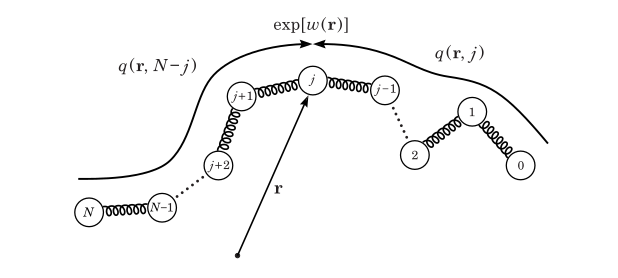
\includegraphics[scale=0.7]{./figures/Figure_1.png}
\end{figure}


































\subsection{单链平均和算子}
\begin{quotation}
在前面的章节中,我们描述了如何使用Chapman-Kolmogorov或Fokker-Planck方程计算单链在外场存在下的分布函数。单链配分函数和约化分布函数(链传播子)是非均匀聚合物理论中的中心对象,有必要将其它“可观测”量表示为外场变量的显式泛函。这主要的量与单链自由度构象全体平均受到外势有关。例如:离散高斯链受到化学势$\omega (\mathbf{r})$的情况下,我们可以定义任何函数$f(\mathbf{r}^{N+1})$珠坐标(bead coordinates)的单链平均:
\end{quotation}
\begin{equation}\label{1}
<f(\mathbf{r}^{N+1})>_{[\omega]}= \frac{\int d \mathbf{r}^{N+1} f(\mathbf{r}^{N+1})exp[-\beta U(\mathbf{r}^{N+1})]}{\int d\mathbf{r}^{N+1}exp[-\beta U(\mathbf{r}^{N+1})]}
\end{equation}
\begin{quotation}
其中$U(\mathbf{r}^{N+1})$是公式(\ref{1})给出的电势。尖括号的下标[w]在对珠坐标进行平均,平均量可以看作是外场$\omega(\mathbf{r})$的函数。同样,对于存在化学势和应变场$\omega(\mathbf{r})$和$\mathbf{\epsilon}$的连续高斯链,相应的单链平均值可以定义为:
\end{quotation}
\begin{equation}\label{2}
<f[\mathbf{r}]>_{[\omega ,\epsilon]}=\frac{\int D\mathbf{r}f[\mathbf{r}]exp(-\beta U_{0}[\mathbf{r}]-\beta U_{1}[\mathbf{r},\omega]-\beta U_{el}[\mathbf{r},\epsilon])}{\int D\mathbf{r}exp(-\beta U_{0}[\mathbf{r}]-\beta U_{1}[\mathbf{r},\omega]-\beta U_{el}[\mathbf{r},\epsilon])}
\end{equation}
\begin{quotation}
其中$f[\mathbf{r}]$是链构型$\mathbf{r}(s)$的任意泛函。
\end{quotation}
\begin{quotation}
主要有趣的单链平均量是段密度、密度相关性和弹性应力,所有这些都可以与非均匀聚合物实验中的可观测值联系起来。我们将看到在某些情况,可以通过取关于场变量$\omega(\mathbf{r})$和$\mathbf{\epsilon}$的规范配分函数$Q[\omega]$和$Q[\omega,\epsilon]$的函数导数来获得这些结果。读者不熟悉函数的变分,建议参考附录C。
\end{quotation}
\subsubsection{密度算子}
\begin{quotation}
首先,我们考虑在化学势$\omega(\mathbf{r})$作用下的单个柔性聚合物的平均段数密度的计算问题。这个数量定义为:
\end{quotation}
\begin{equation}\label{3}
\rho(\mathbf{r};[\omega])\equiv<\hat{\rho}(\mathbf{r})>_{[\omega]}
\end{equation}
\begin{quotation}
其中微观密度$\hat{\rho}(\mathbf{r})$由公式(3.3)或(3.18)给出,这取决于采用的是离散的或连续的高斯链模型。我们将$\rho(\mathbf{r};[\omega])$称为单链密度算子,因为它将平均段密度表示为强加场$\omega$的一个泛函。我们将在第四章中看到,场构造分布合适时,许多聚合物相互作用流体的平均单体密度与算子$\rho(\mathbf{r};[\omega])$的平均值成正比。在这种情况下场不是外部强加的,而是由非键单体之间的相互作用在内部产生的。因此,在多链流体中的“可观测”量的计算将涉及两种不同类型全体平均:(i)公式(\ref{1})和(\ref{2})描述单链的平均;(ii)内部产生电势场分布的场论平均值。关于第二类平均的讨论将推迟到第四章。
\end{quotation}
\begin{quotation}
在计算公式(\ref{3})时,我们再次指出$\omega(\mathbf{r})$和$\hat{\rho}(\mathbf{r})$是热力学共轭变量。因此,$-lnQ[\omega]$泛函关于$\omega(\mathbf{r})$的导数会生成单链$\hat{\rho}(\mathbf{r})$的平均。例如:在离散高斯链的情况下,关于$Q$的公式(3.4)和单链平均定义(\ref{1})。特别是:
\end{quotation}
\begin{equation}\label{4}
-\frac{\delta lnQ[\omega]}{\delta \omega(\mathbf{r})}=-\frac{1}{Q[\omega]}\frac{\delta Q[\omega]}{\delta \omega(\mathbf{r})}=<\hat{\rho(\mathbf{r})}>[\omega]
\end{equation}
\begin{quotation}
因此,段密度算子的另一个表达式是
\end{quotation}
\begin{equation}\label{5}
\rho(\mathbf{r};[\omega])=-\frac{1}{Q[\omega]}\frac{\delta Q[\omega]}{\delta \omega(\mathbf{r})}
\end{equation}
\begin{quotation}
这个表达式的右边可以通过公式(3.6)的泛函微分直接计算(对于离散的高斯链)。这导致:
\end{quotation}
\begin{align}\label{6}
\begin{split}
\frac{\delta Q[\omega]}{\delta \omega(\mathbf{r})}=\frac{1}{V}\sum_{j=0}^{N}\int d\mathbf{r}^{N+1}&[e^{-\omega(\mathbf{r}_{N})}\phi(\mathbf{r}_{N}-\mathbf{r}_{N-1})e^{-\omega(\mathbf{r}_{N-1})}\phi(\mathbf{r}_{N-1}-\mathbf{r}_{N-2}) \\ &\times \ldots e^{-\omega(\mathbf{r}_{j})}(-1)\delta(\mathbf{r}-\mathbf{r}_j)\Phi(\mathbf{r}_j-\mathbf{r}_{j-1})e^{-\omega(\mathbf{r}_j-1)}\\ & \times \ldots e^{-\omega(\mathbf{r}_{2})}\Phi(\mathbf{r}_{2}-\mathbf{r}_{1})e^{-\omega(\mathbf{r}_{1})}\Phi(\mathbf{r}_{2}-\mathbf{r}_{0})e^{-\omega(\mathbf{r}_{0})}]
\end{split}
\end{align}
\begin{quotation}
公式(\ref{6})中的δ函数可以用来消去$\mathbf{r}_{j}$上的积分,即珠 j的位置。这产生了表因式分解的表达示,类似于公式(3.10)描述的的因式分解性质,如图3.1所示。按照同样的推理,可以通过组成传播子$q(\mathbf{r},j;[\omega])$重写公式(\ref{6}),用“互补”传播子$q(\mathbf{r},N-j;[\omega])$描述链段的统计权重,该链段从珠0开始,终止于珠j。后者描述的统计权重与剩余链段相关,从珠N开始,用珠j完成。因此,公式(\ref{6})可以表示为:
\end{quotation}
\begin{equation}\label{7}
\frac{\delta Q[\omega]}{\delta \omega(\mathbf{\mathbf{\mathbf{r}}})}=-\frac{e^{\omega(\mathbf{r})}}{V}\sum_{j=0}^{N}q(\mathbf{r},N-j;[\omega])q(\mathbf{r},j;[\omega])
\end{equation}
\begin{quotation}
因此:	
\end{quotation}
\begin{equation}\label{8}
\rho(\mathbf{r},[\omega])=\frac{e^{\omega}}{VQ[\omega]}\sum_{j=0}^{N}q(\mathbf{r},N-j;[\omega])q(\mathbf{r},j;[\omega])
\end{equation}
\begin{quotation}
方程(\ref{8})是非均匀聚合物理论中的一个重要公式,因为它提供了计算具有任意电势$\omega(\mathbf{r})$的离散高斯链平均段密度的方法。给出$\omega(\mathbf{r})$的表达式,首先递归求解公式(3.8)[在初始条件(3.7)下],得到j=0,1,2,…,N的$q(\mathbf{r},j;[\omega])$。其次,用公式(3.9)计算$Q[\omega]$。这些结果可用于计算公式(\ref{8})右侧的表达式。因此,对所有珠子j的链传播子$q(\mathbf{r},j;[\omega])$的知识足以确定规范化配分函数$q[\omega]$和平均段密度$\rho(\mathbf{r};[\omega])$。
\end{quotation}
\begin{quotation}
这些结果很容易推广到其他链模型中。按照公式(3.21)离散的连续高斯链,连续高斯链类似公式(\ref{8})的模拟量是:
\end{quotation}
\begin{align}\label{9}
\begin{split}
\rho(\mathbf{r},[\omega])&=-\frac{1}{Q[\omega]}\frac{\delta Q[\omega]}{\delta \omega(\mathbf{r})}\\ &=\frac{\triangle s ~exp[\triangle s\omega(\mathbf{r})]}{VQ[\omega]}\sum_{j=0}^{N_s}q(\mathbf{r},(N_s-j)\triangle s;[\omega])q(\mathbf{r},j\triangle s;[\omega])
\end{split}
\end{align}
\begin{quotation}
当取连续极限$N_s\to \infty$,$\triangle s=N/N_s\to 0$,时,我们发现这个表达式可以化简为:
\end{quotation}
\begin{equation}\label{10}
\rho(\mathbf{r},[\omega])=\frac{1}{VQ[\omega]}\int_{0}^{N}ds~q(\mathbf{r},(N-s);[\omega])q(\mathbf{r},s;[\omega])
\end{equation}
\begin{quotation}
这是一个众所周知的结果,是非均匀聚合物的核心理论。其次,我们发现它和连续高斯链(3.27)的因式分解性质相似。
\end{quotation}
\begin{quotation}
密度算子$\rho(\mathbf{r},[\omega])$描述了链段的平均密度,而不是它们沿聚合物的位置。另一个有用的密度算子,例如:连续高斯链是数量:
\end{quotation}
\begin{equation}\label{11}
\rho(\mathbf{r},s;[\omega])\equiv <\hat{\rho}(\mathbf{r},s)>_{[\omega]}
\end{equation}
\begin{quotation}
表示位于等高线位置s的分段的平均密度。用$\hat{\rho}(\mathbf{r},s)=\delta(\mathbf{r}-\mathbf{r}(s))$表示各段在位置s的微观密度。通过引入共轭场$\omega_s(\mathbf{r})$来计算$\hat{\rho}(\mathbf{r},s)$
,仅能计算单体s,并对相互作用能贡献一个附加项:
\end{quotation}
\begin{equation}\label{12}
\beta U_1[\mathbf{r},\omega ,\omega_s]=\int d\mathbf{r}^{'}[\hat{\rho}(\mathbf{r}^{'})\omega (\mathbf{r}^{'})+\hat{\rho}(\mathbf{r}^{'},s)\omega_s(\mathbf{r}^{'})]
\end{equation}
\begin{quotation}
下面的参数类似于公式(\ref{5})的参数,给出结果:
\end{quotation}
\begin{equation}\label{13}
\rho(\mathbf{r},s;[\omega])=<\hat{\rho}(\mathbf{r},s)>_{[\omega]}
=-\frac{\delta lnQ[\omega,\omega_s]}{\delta \omega_s(\mathbf{r})} \bigg |_{\omega_s=0}
\end{equation}
\begin{quotation}
我们现回到$Q[\omega,\omega_s]$的路径积分离散化的步骤,对$\omega_s$微分,并取连续极限。如果令$\omega_s(\mathbf{r})=0$,结果是:
\end{quotation}
\begin{equation}\label{14}
\rho(\mathbf{r},s;[\omega])=\frac{1}{VQ[\omega]}q(\mathbf{r},(N-s);[\omega])q(\mathbf{r},s;[\omega])
\end{equation}
\begin{quotation}
图\ref{figure1}描述了公式(\ref{14})的物理含量,与公式(\ref{10})的比较,我们发现平均总段密度$\rho(\mathbf{r};[\omega])$是所有轮廓位置$0\le s\le N$上的平均段s的密度$\rho(\mathbf{r},s;[\omega])$的简单积分:
\end{quotation}
\begin{figure}[ht]
\centering
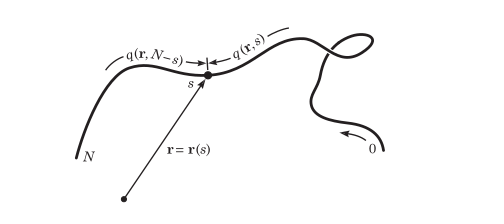
\includegraphics[width=7cm]{./figures/32.png}
\caption{说明位于连续高斯链位置s处的段的平均密度的组成公式(\ref{14})。轮廓长度s的链段的统计权重q(r,s;[w])在点r=r(S)处与具有轮廓长度N−s的基本链段的统计权重q(r,N−s;[w])连接。}
\label{figure1}
\end{figure}
\begin{equation}\label{15}
\rho(\mathbf{r};[\omega])=\int_{0}^{N}ds~\rho(\mathbf{r},s;[\omega])
\end{equation}
\begin{quotation}
该公式与微观密度$\hat{\rho}(\mathbf{r})$和$\hat{\rho}(\mathbf{r},s)$之间的关系有明显的一致性。
\end{quotation}
\begin{quotation}
公式(\ref{14})的一个特例是特别令人感兴趣的。通过设置s=0或s=N,可以得到链端段的平均密度。在目前的均聚物的情况下,两个链端是不可区分的,所以总链端密度可以由
\end{quotation}
\begin{align}\label{16}
\begin{split}
\rho_e(\mathbf{r};[\omega])&\equiv \rho(\mathbf{r},0;[\omega])+\rho(\mathbf{r},N;[\omega])\\  &=\frac{2}{VQ[\omega]}q(\mathbf{r},N;[\omega])
\end{split}
\end{align}
\begin{quotation}
在这个表达式的第二行中,我们使用了$q(\mathbf{r},0;[\omega])=1$。因此,在应用规范化$\frac{2}{VQ[\omega]}$后,传播子$q(\mathbf{r},N;[\omega])$可以解释为链端在r位置的平均密度。
\end{quotation}
\begin{quotation}
公式(\ref{11})-(\ref{16})中的结果可以很容易地推广到离散高斯链模型。为了简洁起见,我们省略简结的概括,转而转向类似蠕虫的链。在类虫链模型,引入了一个场$\omega(\mathbf{r},\mathbf{u})$,它与片段位置和取向的微观密度$\hat{\rho}(\mathbf{r},\mathbf{u})$的共轭。因此,对于段位置和取向密度的单链平均值的算子可以被定义为:
\end{quotation}
\begin{equation}\label{17}
\rho(\mathbf{r},\mathbf{u};[\omega])\equiv <\hat{\rho}(\mathbf{r},\mathbf{u})>_{[\omega]}=-\frac{\delta lnQ[\omega]}{\delta \omega(\mathbf{r},\mathbf{u})}
\end{equation}
\begin{quotation}
这个表达式可以通过离散Q[w]的路径积分、对w(r,u)的微分和恢复连续极限来计算。结果如下:
\end{quotation}
\begin{equation}\label{18}
\rho(\mathbf{r},\mathbf{u};[\omega])=\frac{1}{4\pi VQ[\omega]}\int_{0}^{L_c}ds~ q(\mathbf{r},-\mathbf{u},L_c-s;[\omega])q(\mathbf{r},\mathbf{u},s;[\omega])
\end{equation}
\begin{quotation}
这个表达式类似于因式分解性质(3.41),因为传播子$q(\mathbf{r},-u,L_c-s,[\omega])$描述了“互补”链段的统计权重,其符号为u相反数。
\end{quotation}
\begin{quotation}
从公式(\ref{18})中可以得到几个相关的平均密度。在r或u的两边积分后,得到段方向或位置的平均密度。因此,
\end{quotation}
\begin{align}\label{19}
\begin{split}
\rho(\mathbf{u};[\omega])&\equiv\int d\mathbf{r} \rho(\mathbf{r},\mathbf{u};[\omega]) \\&=\frac{1}{4\pi VQ[\omega]}\int d\mathbf{r} \int_{0}^{L_c}ds~q(\mathbf{r},-\mathbf{u},L_c-s;[\omega])q(\mathbf{r},\mathbf{u},s;[\omega])
\end{split}
\end{align}
\begin{quotation}
和
\end{quotation}
\begin{align}\label{20}
\begin{split}
\rho(\mathbf{r};[\omega])&\equiv\int d\mathbf{u} \rho(\mathbf{r},\mathbf{u};[\omega]) \\&=\frac{1}{4\pi VQ[\omega]}\int d\mathbf{u} \int_{0}^{L_c}ds~q(\mathbf{r},-\mathbf{u},L_c-s;[\omega])q(\mathbf{r},\mathbf{u},s;[\omega])
\end{split}
\end{align}
\begin{quotation}
提供关于分段位置和位置分布的单独信息。我们还可以避免公式(\ref{18})中的链轮廓积分,从而导出在指定等高线位置s处分段位置和方向的平均密度公式为:
\end{quotation}
\begin{equation}\label{21}
\rho(\mathbf{r},\mathbf{u};[\omega])=\frac{1}{4\pi VQ[\omega]}q(\mathbf{r},-\mathbf{u},L_c-s;[\omega])q(\mathbf{r},\mathbf{u},s;[\omega])
\end{equation}
\begin{quotation}
最后,该表达式可用于推导出链端段位置和方向的平均密度。
\end{quotation}
\begin{align}\label{22}
\begin{split}
\rho_e(\mathbf{r},\mathbf{u};[\omega])&\equiv\rho(\mathbf{r},\mathbf{u},0;[\omega])+\rho(\mathbf{r},\mathbf{u},L_c;[\omega])\\ &=\frac{1}{4\pi VQ[\omega]}[q(\mathbf{r},-\mathbf{u},L_c;[\omega])+q(\mathbf{r},\mathbf{u},L_c;[\omega])]
\end{split}
\end{align}
\begin{quotation}
对于棒状聚合物模型,段位置和取向的密度算子与蠕虫链的密度算子一致。见公式(\ref{17})。采用公式(3.45)的一阶泛函导数将导致:
\end{quotation}
\begin{equation}\label{23}
\rho(\mathbf{r},\mathbf{u};[\omega])=\frac{1}{4\pi VQ[\omega]}\int_{0}^{L_c}ds~exp[-\int_{0}^{L_c}ds^{'}\omega (\mathbf{r}+(s^{'}-s)\mathbf{u},\mathbf{u})]
\end{equation}
\begin{quotation}
通过定义棒状聚合物的传播子q(r,u,s;[w])
\end{quotation}
\begin{equation}\label{24}
q(\mathbf{r},\mathbf{u},s;[\omega])\equiv exp[-\int_{0}^{s}ds^{'}\omega(\mathbf{r}-s^{'}\mathbf{u},\mathbf{u})]
\end{equation}
\begin{quotation}
假设w(r,u)=w(r,−u),则公式(\ref{23})中给出的棒状聚合物密度算子可以与公式(\ref{18})蠕虫链的表示形式完全相同。
\end{quotation}
\begin{quotation}
单链密度算子范畴下的最后一个话题是段密度的高阶矩。对象Q[w]和ln Q[w]可视为生成泛函(Van Kampen1981),因为这些量的泛函导数分别产生了微观单链密度的矩和累积量(见附录B)。实际上,对于高斯链模型,我们已经看到第一时刻有交替的表示。
\end{quotation}
\begin{equation}\label{25}
<\hat{\rho}(\mathbf{r})>_{[\omega]}=-\frac{\delta lnQ[\omega]}{\delta \omega(\mathbf{r})}=-\frac{1}{Q[\omega]}\frac{\delta Q[\omega]}{\delta\omega(\mathbf{r})}
\end{equation}
\begin{quotation}
同样地,从规范化的配分函数和单链平均的定义中看出,微观密度的第二矩是由Q的第二泛函导数给出的。
\end{quotation}
\begin{equation}\label{26}
<\hat{\rho}(\mathbf{r})\hat{\rho}(\mathbf{r}^{'})>_{[\omega]}=\frac{1}{Q[\omega]}\frac{\delta^2 Q[\omega]}{\delta\omega(\mathbf{r})\delta \omega(\mathbf{r}^{'})}
\end{equation}
\begin{quotation}
第二累积矩同样由lnQ的第二泛函导数来表示:
\end{quotation}
\begin{equation}\label{27}
<\hat{\rho}(\mathbf{r})\hat{\rho}(\mathbf{r}^{'})>_{[\omega]}-<\hat{\rho}(\mathbf{r})>_{[\omega]}<\hat{\rho}(\mathbf{r}^{'})>_{[\omega]}=\frac{\delta^2 lnQ[\omega]}{\delta\omega(\mathbf{r})\delta \omega(\mathbf{r}^{'})}
\end{equation}
\begin{quotation}
我们回顾了公式(\ref{8})和(\ref{10})给出了链传播子q与微观段密度的第一矩之间高斯链模型的明确关系。传播子和矩之间的这种联系可以扩展到高阶矩,方法是采用附加的函数导数,从而在附加点上考虑链的统计权重。例如,在连续高斯链的情况下,二阶矩,或密度-密度相关函数,给出:
\end{quotation}
\begin{align}\label{28}
\begin{split}
<\hat{\rho}(\mathbf{r})\hat{\rho}(\mathbf{r}^{'})>_{[\omega]}&=\frac{1}{VQ[\omega]}\int_{0}^{N}ds \int_{0}^{s}ds^{'}q(r,N-s;[\omega])\\&\times g(\mathbf{r},\mathbf{r}^{'},s-s^{'};[\omega])q(\mathbf{r}^{'},s^{'};[\omega])\\&+\frac{1}{VQ[\omega]}\int_{0}^{N}ds^{'} \int_{0}^{s^{'}}ds^{'}q(\mathbf{r}^{'},N-s^{'};[\omega])\\&\times g(r^{'},\mathbf{r},s^{'}-s;[\omega])q(\mathbf{r},s;[\omega])
\end{split}
\end{align}
\begin{quotation}
这个方程中出现的函数$g(\mathbf{r},s,[\omega])$是一个新的链传播子,它满足公式(3.25),但服从$\delta$函数初始条件,即:
\end{quotation}
\begin{equation}\label{29}
\frac{\partial}{\partial s}g(\mathbf{r},\mathbf{r}^{'},s;[\omega])=\frac{b^2}{6}\bigtriangledown^2g(\mathbf{r},\mathbf{r}^{'},s;[\omega])-\omega(\mathbf{r})g(\mathbf{r},\mathbf{r}^{'},s;[\omega])
\end{equation}
\begin{equation}\label{30}
g(\mathbf{r},\mathbf{r}^{'},0;[\omega])=\delta(\mathbf{r}-\mathbf{r}{'})
\end{equation}
\begin{quotation}
因此,$g(\mathbf{r},\mathbf{r}^{'},s;[\omega])$是公式(3.25)的格林函数(或基本)解,如图\ref{figure2}所示,这个传播子生成聚合物的长度s内部截面的统计权重,它起源于r位,终止于r位置。
\end{quotation}
\begin{figure}[h]
\centering
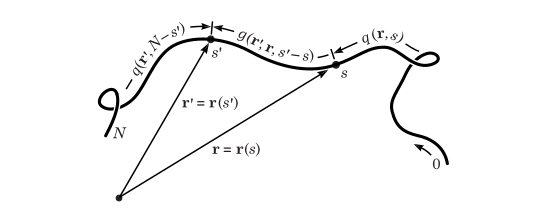
\includegraphics[width=7cm]{./figures/33.png}
\caption{解释了连续高斯链段密度-密度相关函数的合成公式(\ref{28})(仅最后一项)。轮廓长度-s的链端截面的统计权重$q(\mathbf{r},s)$在点$\mathbf{r}=\mathbf{r}(s)$处连接到传播子$g(\mathbf{r}^{'},\mathbf{r},s^{'}-s)$。传播子描述与长度为$s^{'}-s$的内部链段相关的统计权重,从$\mathbf{r}=\mathbf{r}(s^{'})$开始,结束于$r=r(s)$。最后“互补”链端截面的统计权重为$q(\mathbf{r},N-s^{'})$。}
\label{figure2}
\end{figure}
\begin{quotation}
图\ref{figure2}描述了公式(\ref{27})的物理解释。该方程可用于计算具有势$\omega(\mathbf{r})$的连续高斯链段密度的二阶矩。虽然这类高阶密度相关函数的公式便于近似解析计算,但在高分辨率的数值工作中应避免。这是因为计算两点传播子(如$g(\mathbf{r},s,[\omega])$所付出的代价)。如果使用M个网格点或谱分量来求解空间自由度,请参见第3.6节,g的数值计算至少需要$M^2$算子。在三维模拟中, 使用这样的$O(M^2)$缩放的计算令人望而却步, 其中M大到$10^6-10^7$.
\end{quotation}
\subsubsection{应力算子(Stress operators)}
\begin{quotation}
另一个重要的量是放置在不均匀环境中的聚合物链所产生的平均弹性应力。弹性应力算子可以定义为
\end{quotation}
\begin{equation}\label{31}
\sigma(\mathbf{\mathbf{r}};[\omega,\epsilon])\equiv<\hat{\sigma}(\mathbf{r})>_{[\omega,\epsilon]}
\end{equation}
\begin{quotation}
其中,单链平均是根据公式(\ref{2})计算的。用离散高斯链模型计算这个表达式的右边会产生两个不同的表达式,
\end{quotation}
\begin{align}\label{32}
\begin{split}
\sigma(\mathbf{r};[\omega,\epsilon])&=\frac{\int d\mathbf{r}^{N+1}\hat{\sigma}(\mathbf{r})exp[-\beta U(\mathbf{r}^{N+1})-\beta U_{el}(\mathbf{r}^{N+1})]}{\int d\mathbf{r}^{N+1}exp[-\beta U(\mathbf{r}^{N+1})-\beta U_{el}(\mathbf{r}^{N+1})]}\\&=\frac{\int d\mathbf{r}^{N+1}\hat{\sigma}(\mathbf{r})exp[-\beta U(\mathbf{r}^{N+1})-\beta U_{el}(\mathbf{r}^{N+1})]}{Q[\omega,\epsilon]\int d\mathbf{r}^{N+1}exp[-\beta U_0(\mathbf{r}^{N+1})-\beta U_{el}(\mathbf{r}^{N+1})]}
\end{split}
\end{align}
\begin{quotation}
第二个是最方便计算的。在最后一个表达式中插入微观应力运算符公式(3.11)的显式形式将导致:
\end{quotation}
\begin{equation}
\begin{aligned}\label{33}
\sigma_{\alpha \gamma}(\mathbf{r};[\omega,\epsilon])&=\frac{3k_BT}{b^2VQ[\omega,\epsilon]} \int d\mathbf{r}^{'}(\mathbf{r}^{'}-\mathbf{r})_{\alpha} (\mathbf{r}^{'}-\mathbf{r})_{\gamma} \varPsi (\mathbf{r}^{'}-\mathbf{r};[\epsilon])\\&\times \sum_{j=0}^{N-1}q(\mathbf{r}^{'},N-j-1;[\omega,\epsilon])q(\mathbf{r},j;[\omega,\epsilon])
\end{aligned}
\end{equation}
\begin{quotation}
其中函数$\varPsi (\mathbf{r}^{'}-\mathbf{r};[\epsilon])$是在公式(3.14)中定义的。这个表达式可以通过先解公式(3.15)-(3.17)得到传播子$q(\mathbf{r},j;[\omega,\epsilon])$和配分函数$Q[\omega,\epsilon]$然后指定公式(\ref{33})中的被积和求和,其余操作可以数值执行。
\end{quotation}
\begin{quotation}
在连续高斯链模型的基础上,导出了应力算子的类似表达式(Fredrickson,2002)。对于非均匀应变场,这个表达式是相当复杂的,因此不在这里再现。在均质菌株的情况下,得到$^{19}$.
\end{quotation}
\begin{equation}\label{34}
\sigma(\mathbf{r};[\omega,\epsilon])=\frac{3k_BT}{b^2VQ[\omega,\epsilon]}\int_{0}^{N} ds~q(r,s;[\omega,\epsilon])\nabla \nabla q(\mathbf{r},N-s;[\omega,\epsilon])
\end{equation}
\begin{quotation}
应力算符的这个表达式表明,在空间变化的化学势$\omega(\mathbf{r})$存在下,弹性应力是各向异性的和非均匀的。应力各向异性是由沿链等高线积分的并矢量$q\nabla \nabla q$来表示的。泰勒和莫尔斯在研究嵌段共聚物中间相的线弹性性质时,推导出了密切相关的公式(Tyler and morse,2003a;Tyler and Morse,2003b)。方程(\ref{34})对于研究细观结构聚合物流体中链拉伸的不均匀分布特别有用。
\end{quotation}

\subsection{其他的结构}
前一节假设了最简单的聚合物结构-线性均聚物。对于各种各样的体系结构包括那些具有实际和学术意义的体系都可以得到类似的结果。在本节中,我们导出了在空间变化势作用下分支均聚物(branched homopolymers)、嵌段共聚物和接枝共聚物(block and graft copolymers)的显式表达式。假定聚合物的结构是化学无序的,如随机分支均聚物(randomly branched homoploymers)、统计共聚物(statistical copolymers)和随机接枝共聚物(randomly grafted copolymers)的讨论,将推迟到$4.7$节讨论。
\subsubsection{分支均聚物}
作为分支均聚物的第一个例子,我们考虑一个$3$臂星形均聚物,如图\ref{三臂星形均聚物}所示。每个臂采用连续高斯链模型描述并且有任意的长度。相应的,每条链的聚合度分别是$N_1$,$N_2$,$N_3$。假设每个臂上的片段经历一个化学势场$w (\mathbf{r})$。在这种情况下只需要一种化学势,因为每个臂是相同的。
\begin{figure}[H]
\centering
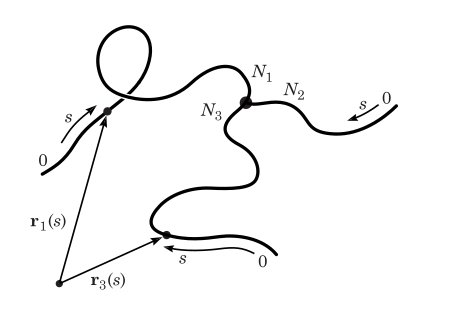
\includegraphics[scale=0.7]{./figures/34.png}
\caption{连续高斯链模型中的$3$臂星形聚合物。聚合度分别为$N_1$,$N_2$,$N_3$的三个支臂连接在一个中心支点上。第$j$个臂的构型用空间曲线$\mathbf{r}_j(s)$描述,$s\in [0,N_j]$。}
\label{三臂星形均聚物}
\end{figure}

如图\ref{三臂星形均聚物}所示,第$j$个臂$(j=1,2,3)$的构型由空间曲线$\mathbf{r}_j(s)$描述,其中路径参数$0\leq s\leq N_j$,这是从每个臂的自由端测量。在支点处,臂满足$\mathbf{r}_1(N_1)=\mathbf{r}_2(N_2)=\mathbf{r}_3(N_3)$。

第$3.1.2$节关于线性均聚物的公式可以很容易地推广到目前的情况。微观段密度(microscopic segment density)可以写成
\begin{equation}
\hat{\rho}(\mathbf{r})=\sum_{j=1}^3 \int_{0}^{N_j}\, \mathrm{d}s\rho(\mathbf{r}-\mathbf{r}_{j}(s))
\end{equation}
与施加的化学势$w (\mathbf{r})$的相关的势能是整个聚合物形状$\mathbf{r}$的一个泛函,$\mathbf{r}(s)\equiv \left\{ \mathbf{r}_1(s),\mathbf{r}_2(s),\mathbf{r}_3(s) \right\}:$
\begin{equation}
\beta U_1[\mathbf{r},w]=\int \mathrm{d}\mathbf{r}^{'}w(\mathbf{r}^{'})\hat{\rho}(\mathbf{r}^{'})
\end{equation}
归一化的配分函数$Q[w]$也可以表示为路径积分的比率
\begin{equation}
Q[w]\equiv \frac{Z[w]}{Z_0}=\frac{\int^{*}\mathcal{D}\mathbf{r}\exp (-\beta U_0[\mathbf{r}]-\beta U_1[\mathbf{r},w])}{\int^{*}\mathcal{D}\mathbf{r}\exp (-\beta U_0[\mathbf{r}])} \label{82}
\end{equation}
其中理想链的势能
\begin{equation}
\beta U_0[\mathbf{r}]=\frac{3}{2b^2}\sum_{j=1}^3\int_{0}^{N_j} \mathrm{d}s\left| \frac{d\mathbf{r}_j(s)}{ds} \right|^2
\end{equation}
和$\int^{*}\mathcal{D}\mathbf{r}$是受支点约束的三个臂上的路径积分
\begin{equation}
\int^{*}\mathcal{D}\mathbf{r}\equiv \int \mathcal{D}\mathbf{r}\delta (\mathbf{r}_1(N_1)-\mathbf{r}_2(N_2))\delta (\mathbf{r}_2(N_2)-\mathbf{r}_3(N_3))  \label{83}
\end{equation}
方程(\ref{82})中的路径积分可以通过离散这三条路径来计算,这三条路径对应于星臂的构型,从而得到了一个类似于线性均聚物方程$(3.21)$的表达式。方程(\ref{83})的约束是通过建立从三个臂的自由端开始,在公共分支点的位置终止的路径积分,因此,由乘积$q(\mathbf{r},N_1)q(\mathbf{r},N_2)q(\mathbf{r},N_3)$给出了有支点的星形聚合物关于$\mathbf{r}$的统计重量,其中传播子(propagators)满足方程$(3.25)-(3.26)$。配分函数是
\begin{equation}
Q[w]=\frac{1}{V}\int \mathrm{d}\mathbf{r}~q(\mathbf{r},N_1;[w])q(\mathbf{r},N_2;[w])q(\mathbf{r},N_3;[w])
\end{equation}
应该注意,应用这个公式并不需要扩散方程$(3.25)$的三个独立解,而是一个,因为对$0\leq s\leq N_{\max}$(其中$N_{\max}$是$N_j$中最大的)的$q(\mathbf{r},s;[w])$足以评估全部的三个传播子。

$3$臂星形均聚物的段密度算子可与线性聚合物的方程$(3.55)$类比得出。在连续高斯链模型中,我们有
\begin{equation}
\rho(\mathbf{r};[w])=-\frac{1}{Q[w]}\frac{\delta Q[w]}{\delta w(\mathbf{r})}=\rho _1(\mathbf{r};[w])+\rho _2(\mathbf{r};[w])+\rho _3(\mathbf{r};[w])
\end{equation}
这里的$\rho _j(\mathbf{r};[w])$表示星的第$j$个臂对平均段密度的贡献。其中
\begin{equation}
\rho _{j}(\mathbf{r};[w])=\frac{1}{VQ[w]} \int_{0}^{N_j}\, \mathrm{d}s\,q_{j}(\mathbf{r},N_{j}-s;[w])q(\mathbf{r},s;[w]) \label{87}
\end{equation}
“互补传播子”$q_{j}(\mathbf{r},s;[w])$满足与$q$相同的扩散方程,但具有不同的初始条件,即
\begin{equation}
\frac{\partial}{\partial s}q_j(\mathbf{r},s;[w])=\frac{b^2}{6}q_j(\mathbf{r},s;[w])-w(\mathbf{r})q_j(\mathbf{r},s;[w]) \label{88}
\end{equation}
\begin{equation}
q_j(\mathbf{r},0;[w])=
\begin{cases}
q(\mathbf{r},N_2;[w])q(\mathbf{r},N_3;[w]), & j=1 \\
q(\mathbf{r},N_1;[w])q(\mathbf{r},N_3;[w]), & j=2 \\
q(\mathbf{r},N_1;[w])q(\mathbf{r},N_2;[w]), & j=3  \label{89}
\end{cases}
\end{equation}

\begin{figure}[H]
\centering
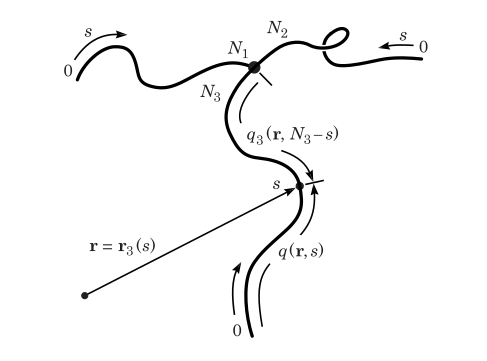
\includegraphics[scale=0.7]{./figures/35.png}
\caption{$3$臂星形均聚物的密度算子$\rho _3(\mathbf{r};[w])$的构造。这个密度由统计权重$q(\mathbf{r},s;[w])$组成,代表臂$3$的自由端,具有互补的传播子$q_3(\mathbf{r},N_3-s;[w])$,表示臂与分支点连接的部分的统计重量。在满足初始条件(\ref{89}),后者是通过对远离分支点的方程(\ref{88})进行积分获得的。}
\label{三臂星形图像}
\end{figure}

图(\ref{三臂星形图像})说明了当$j=3$时的臂的平均密度$\rho _3$的方程(\ref{87})的物理解释。臂必须通过点$\mathbf{r}=\mathbf{r}_3(s)$,其中$s$是从臂的自由端测量的路径参数。与这种臂构型相关联的是统计重量$q(\mathbf{r},s;[w])$的乘积,它表示臂的悬空(自由)末端,以及重量$q_{3}(\mathbf{r},N_{3}-s;[w])$,表示与星其余部分相连的臂段。互补传播子$q_3$是从分支点开始,在$N_3-s$的总的路径距离上对方程(\ref{88})积分得出的。这种积分的初始条件是在分支点与剩余的两个臂相关联的统计权重,它可以用两个$q$传播子的乘积表示,如方程(\ref{89})所述。

上述结果可以很容易地推广到具有任意臂数的星均聚物。最一般情况是具有不同长度且$p\geq3$臂的星,总段密度算子的求值要求扩散方程的$p+1$个解:一种是从长度为$N_{\max}$(最长臂长)的链获得$q$,另一解为$p$互补传播子$q_j(\mathbf{r},s;[w])$,$s\in [0,N_j]$。在具有等臂长的$p$星聚合物的特殊情况下,由于所有互补传播子相同,计算量大大减少。因此,在这种高对称性的特殊情况下,只需要扩散方程的两个解。

\begin{figure}[H]
\centering
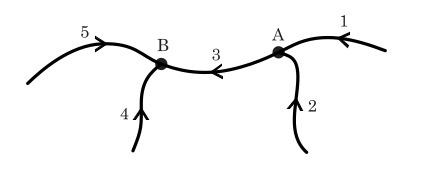
\includegraphics[scale=0.7]{./figures/36.png}
\caption{另一个例子,一个分支均聚物由$5$部分组成,$1-5$连接在两个分支点$A$和$B$上。箭头表示一个(任意)的积分方向,以建立聚合物的统计重量。}
\label{AB嵌段}
\end{figure}

作为分支均聚物的第二个例子,我们考虑了图(\ref{AB嵌段})所示的支化聚合物。聚合物由标记为$1-5$的五个节段组成,分别连接在$A$和$B$的两个支点处。第$j$节的聚合度用$N_j$表示。没有什么特殊的方法来建立这样一种聚合物的统计重量,但各种替代品提供了同等的结果。为了说明如何通过在分支点$B$处合成传播子来计算归一化配分函数$Q[w]$,图(\ref{AB嵌段})中聚合物截面上的箭头指示了用于计算传播子的积分方向,箭头是任意分配的。有图明显看出,在$B$处,三个方向都聚焦在此,通过将第$3$,$4$和$5$节中的传播子组合在一起可以得到$Q[w]$
\begin{equation}
Q[w]=\frac{1}{V}\int \mathrm{d}\mathbf{r}q_3(\mathbf{r},N_3;[w])q(\mathbf{r},N_4;[w])q(\mathbf{r},N_5;[w])
\end{equation}
第$4$节和第$5$节中,$q$传播子在自由链端开始,因此满足方程$(3.25)-(3.26)$。相反,第3节的$q_3$传播子在分支点$A$处开始,从而满足初始条件下的扩散方程(\ref{88})
\begin{equation}
q_3(\mathbf{r},0;[w])=q(\mathbf{r},N_1;[w])q(\mathbf{r},N_2;[w])
\end{equation}
这个初始条件提供了与支点$A$处的链节$1$和$2$相关联的统计权重。

类似的表达式可以写成对这种支化聚合物的平均段密度的各种贡献。例如,第$3$节对段密度运算符的贡献可以表示为
\begin{equation}
\rho(\mathbf{r};[w])=\frac{1}{VQ[w]}\int _{0}^{N_3} \mathrm{d}sq_{3c}(\mathbf{r},N_3-s;[w])q_3(\mathbf{r},s;[w])
\end{equation}
其中$q_3(\mathbf{r},s;[w])$是从分支点$A$出发的传播子。“互补”传播子$q_{3c}(\mathbf{r},N_3-s;[w])$在分支点$B$处发起,并扩展路径距离$N_3-s$在$\mathbf{r}$点加入传播子$q_{3c}$。在初始条件下,$q_{3c}$满足方程(\label{传播子求导})
\begin{equation}
q_{3c}(\mathbf{r},0;[w])=q(\mathbf{r},N_4;[w])q(\mathbf{r},N_5;[w])
\end{equation}
它提供了分支点$B$处的分支$4$和$5$的统计权重。

利用相关的参数,可以构造具有外势的任意结构的分支均聚物的配分函数以及密度和压力算子。这种表达式也可以推广到连续高斯链之外,在离散和蠕虫状链模型的背景下处理分支聚合物。

\subsubsection{嵌段接枝共聚物}
嵌段共聚物和接枝共聚物是聚合物工业中特别重要的材料,与纳米技术特别相关。由于这种聚合物是由两个或两种以上的在化学性质上不同的部分(“块”或“移植物”)组成的,它们在势场存在的情况下的统计力学比均聚物更丰富。

我们首先讨论$AB$二嵌段共聚物的连续高斯链模型,如图$3.7$所示。共聚物的总聚合物度指数为$N$,$0\leq s \leq fN$(实线)段由$A$型段组成,$fN \leq s \leq N$(虚线)由B型段组成。$f$是表示$A$链长度与总链长度之比的参数,如果进一步定义$A$和$B$段具有相等的体积,则$f$对应于链上$A$型段的平均体积分数。与共聚物的$A$和$B$段相对应的统计段长度分别是$b_A$和$b_B$。我们还引入了外部化学势场$w_A(\mathbf{r})$和$w_B(\mathbf{r})$,它们分别作用于共聚物的$A$和$B$段。

\begin{figure}[H]
\centering
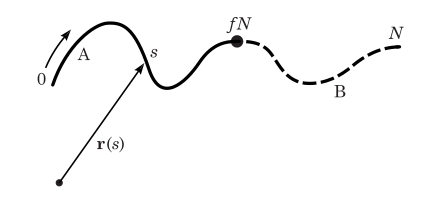
\includegraphics[scale=0.7]{./figures/37.png}
\caption{$AB$二嵌段共聚物的连续高斯链模型。$0\leq s \leq fN$(实线)段由$A$型段组成,$fN \leq s \leq N$(虚线)由$B$型段组成。$f$是表示$A$链长度与总链长度之比的参数。}
\end{figure}

这种二嵌段共聚物的拉伸势能可以表示为
\begin{equation}
\beta U_0[\mathbf{r}]=\int_{0}^{N} \mathrm{d}s\frac{3}{2[b(s)]^2}\left| \frac{d\mathbf{r}(s)}{ds} \right|^2
\end{equation}
这里
\begin{equation}
b(s)\equiv
\begin{cases}
b_A, & 0\leq s \leq fN \\
b_B, & fN \leq s \leq N\\
\end{cases}
\end{equation}
同样,与外部势$w_A$和$w_B$相关的势能可以写为
\begin{equation}
\beta U_1[\mathbf{r},w_A,w_B]=\int \mathrm{d}\mathbf{r}^{'}[w_A(\mathbf{r}^{'})\hat{\rho}_{A}(\mathbf{r}^{'})+w_B(\mathbf{r}^{'})\hat{\rho}(\mathbf{r}^{'})]
\end{equation}
其中$\hat{\rho} _A$和$\hat{\rho} _B$是由下面公式定义的微观段密度
\begin{equation}
\hat{\rho} _A(\mathbf{r})=\int _0^{fN} \mathrm{d}s~\delta(\mathbf{r}-\mathbf{r}(s)),~~~\hat{\rho} _B(\mathbf{r})=\int _{fN}^{N} \mathrm{d}~s\delta(\mathbf{r}-\mathbf{r}(s))
\end{equation}
此二嵌段的归一化配分函数表达式是
\begin{equation}
Q[w_A,w_B]\equiv\frac{Z[w_A,w_B]}{Z_0}=\frac{\int \mathcal{D}\mathbf{r}~\exp(-\beta U_0[\mathbf{r}]-\beta U_1[\mathbf{r},w_A,w_B])}{\int \mathcal{D}\mathbf{r}~\exp(-\beta U_0[\mathbf{r}])}
\end{equation}
前几节所描述的方法也可于将分配函数、密度和压力算子与满足Fokker-Planck方程的链传播算子联系起来。在这种情况下,由共聚物的$s=0$(A块)端引发的传播子$q(\mathbf{r},s;[w_A,w_B])$满足扩散方程
\begin{equation}
\frac{\partial}{\partial s}q(\mathbf{r},s;[w_A,w_B])=\frac{[b(s)]^2}{6}\triangledown ^2q(\mathbf{r},s;[w_A,w_B])-w(\mathbf{r},s)q(\mathbf{r},s;[w_A,w_B]) \label{3.99}
\end{equation}
这里
\begin{equation}
w(\mathbf{r},s)\equiv
\begin{cases}
w_A(\mathbf{r}), & 0\leq s \leq fN \\
w_B(\mathbf{r}), & fN \leq s \leq N\\
\end{cases}
\end{equation}
方程(\ref{3.99})在初始条件$q(\mathbf{r},0;[w_A,w_B])=1$的情况下求解。

另一个有用的量是从共聚物的$s=N$末端出发的互补传播子$q_c(\mathbf{r},s;[w_A,w_B])$。通过建立从$B$端开始的共聚物统计重量,可以直观地证明$q_c$满足类似的扩散方程
\begin{equation}
\frac{\partial}{\partial s}q_c(\mathbf{r},s;[w_A,w_B])=\frac{[b_c(s)]^2}{6}\triangledown ^2q_c(\mathbf{r},s;[w_A,w_B])-w_c(\mathbf{r},s)q_c(\mathbf{r},s;[w_A,w_B]) \label{101}
\end{equation}
这里
\begin{equation}
b_c (s)\equiv
\begin{cases}
b_B, & 0\leq s \leq (1-f)N \\
b_A, & (1-f)N \leq s \leq N\\
\end{cases}
\end{equation}
和
\begin{equation}
w_c (\mathbf{r},s)\equiv
\begin{cases}
w_B(\mathbf{r}), & 0\leq s \leq (1-f)N \\
w_A(\mathbf{r}), & (1-f)N \leq s \leq N\\
\end{cases}
\end{equation}
用$q_c(\mathbf{r},0;[w_A,w_B])=1$,方程(\ref{101})在$s$中也是向前积分的。		

使用上面的传播子,可以用两种等效的方法计算配分函数:
\begin{equation}
\begin{aligned}
Q[w_A,w_B] & = \frac{1}{V}\int \mathrm{d}\mathbf{r}q(\mathbf{r},N;[w_A,w_B]) \\
&=\frac{1}{V}\int \mathrm{d}\mathbf{r}q_c(\mathbf{r},N;[w_A,w_B]) \\
\end{aligned}	
\end{equation}
换句话说,二嵌段共聚物的传播子可以从分子的$A$端或$B$端建立,从而得到整个链的等效统计重量。因此,只需求解方程(\ref{3.99})或方程(\ref{101})就能计算配分函数$Q[w_A,w_B]$。

相反,计算二嵌段共聚物的密度算子需要两个链传播子的信息。$A$段和$B$段的平均密度是由现在熟悉的前向和后向传播子组成的过程构造的,从而得到表达式
\begin{equation}
\begin{aligned}
\rho _A(\mathbf{r};[w_A,w_B]) & =-\frac{1}{Q[w_A,w_B]}	\frac{\delta Q[w_A,w_B]}{\delta w_A(\mathbf{r})} \\
& =\frac{1}{VQ[w_A,w_B]} \int _{0}^{fN}\,\mathrm{d}s~q_c(\mathbf{r},N-s;[w_A,w_B])q(\mathbf{r},s;[w_A,w_B]) \\
\end{aligned}	
\end{equation}

\begin{equation}
\begin{aligned}
\rho _B(\mathbf{r};[w_A,w_B]) & =-\frac{1}{Q[w_A,w_B]}	\frac{\delta Q[w_A,w_B]}{\delta w_B(\mathbf{r})} \\
& \frac{1}{VQ[w_A,w_B]} \int _{fN}^{N}\,\mathrm{d}s~q_c(\mathbf{r},N-s;[w_A,w_B])q(\mathbf{r},s;[w_A,w_B]) \\
\end{aligned}	
\end{equation}
上述结果在嵌段共聚物理论中都是众所周知的(Helfand and Wasserman,1976;Hong and Noolandi,1981;Matsen和Schick,1994a)。

作为最后一个例子,我们讨论$A_2B$接枝共聚物的情况,其结构如图(\ref{3.8})所示。这样的分子可以被看作是有一个$A$主链与一个单一的B块“嫁接”到它。或者,该共聚物可以被看作是一种星共聚物有两个$A$臂,分别是$A_1$和$A_2$,和一个$B$臂。从后一种观点出发,分别用$N_{A1}$,$N_{A2}$和$N_B$来表示臂的聚合程度。为了简单起见,采用了连续高斯链模型。

\begin{figure}[H]
\centering
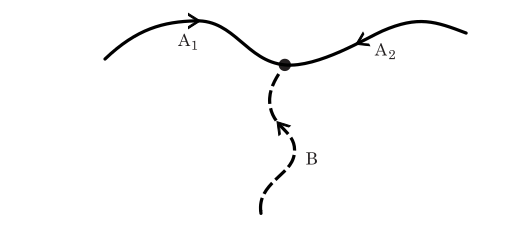
\includegraphics[scale=0.7]{./figures/38.png}
\caption{一个$A_2B$接枝共聚物的连续高斯链模型。该共聚物可视为$B$均聚物链接枝到均聚物主链(实线)$A$上,也可视为具有两个$A$臂和$1$个$B$臂的星共聚物。箭头表示建立该分子的统计重量一个特定(任意)方向。}
\label{3.8}
\end{figure}		

我们需要两个不同的链传播子来构造图(\ref{3.8})所示的接枝共聚物的配分函数$Q[w_A,w_B]$。它们对应于从共聚物臂的自由端开始生长一段$A$或$B$型均聚物链。传播子$q_A(\mathbf{r},s;[w_A])$和$q_A(\mathbf{r},s;[w_A])$满足
\begin{equation}
\frac{\partial}{\partial s}q_K(\mathbf{r},s;[w_K])=\frac{b_K^2}{6}\triangledown ^2q_K(\mathbf{r},s;[w_K])-w_K(\mathbf{r})q_K(\mathbf{r},s;[w_K]) \label{107}
\end{equation}
上式$K=A$或$B$.方程(\ref{107})的求解条件是$q_K(\mathbf{r},0;[w_K])=1$。有了这些定义,接枝共聚物的总统计重量是通过在分支点上连接三个这样的传播子来构造的,这意味着配分函数可以写成
\begin{equation}
Q[w_A,w_B]=\frac{1}{V}\int \mathrm{d}\mathbf{r}~q_A(\mathbf{r},N_{A1};[w_A])q_A(\mathbf{r},N_{A2};[w_A])q_B(\mathbf{r},N_B;[w_B])
\end{equation}

密度算子可以用类似于分支均聚物和二嵌段共聚物的方法来构造.例如,通过将(正前)$B$传播子$q_B$与从支点发起的互补(向后)$B$传播子$q_{B_c}(\mathbf{r},s;[w_A,w_B])$组合,可获得接枝共聚物的平均段$B$密度。后一个传播子满足
\begin{equation}
\frac{\partial}{\partial s}q_{B_c}(\mathbf{r},s;[w_A,w_B])=\frac{b_B^2}{6}\triangledown ^2q_{B_c}(\mathbf{r},s;[w_A,w_B])-w_B(\mathbf{r},s)q_{B_c}(\mathbf{r},s;[w_A,w_B])
\end{equation}
满足
\begin{equation}
q_{B_c}(\mathbf{r},0;[w_A,w_B])=q_A(\mathbf{r},N_{A1};[w_A])q_A(\mathbf{r},N_{A2};[w_A])
\end{equation}
这个初始条件提供了在支点的两个$A$臂的统计重量。在此基础上,$A_2B$接枝共聚物$B$段的平均密度是
\begin{equation}
\begin{aligned}
\rho _B(\mathbf{r};[w_A,w_B]) & =-\frac{1}{Q[w_A,w_B]}	\frac{\delta Q[w_A,w_B]}{\delta w_B(\mathbf{r})} \\
&= \frac{1}{VQ[w_A,w_B]} \int _{0}^{N_B}\,\mathrm{d}s~q_{B_c}(\mathbf{r},N_B-s;[w_A,w_B])q_B(\mathbf{r},s;[w_B]) \\
\end{aligned}	
\end{equation}
对于两个$A$形臂中任何一个$A$形臂所贡献的类型段的平均密度,也可以编写类似的表达式。

\subsection{近似方案}
在本章前三节中,重点关注的是推导外势作用下单链模型配分函数的精确表达式以及平均性质.大多数情况下,这些表达式并不适合进行精确分析.虽然完整的数值解非常重要,但若能得到一些近似解析表达式
(比如配分函数$Q[w]$和密度算子$\rho(\br ;[w])$的近似解析式)也非常有帮助.这些可用于聚合物流体的多链场理论的分析研究.更重要的,理解单链平均值和算子的渐近行为可以帮助发展多链场理论的有效数值方法.

本节将集中讨论推导配分函数和单链平均值的系统扰动展开的方法.这种渐近方法最直接地应用于Fokker-Planck方程可用的连续链模型.因此,对于连续高斯链和类虫链,可以利用偏微分方程正则摄动和奇异摄动方法的大量文献.在本节中,我们将注意力限制在连续链模型上,并尝试提供一个微扰展开的指南.
\subsection{弱非均匀性展开}
当应用的势场$w$具有振幅较弱的不均匀性时,可以得到一个有用的微扰展开式.

为了定义此情形,引入势的体积平均值:
\begin{equation}
w_0\equiv \frac{1}{V} \int w(\br )\,\mathrm{d}\br 
\end{equation}
并重新定义$w(\br )$:
\begin{equation}
w(\br )=w_0+\omega(\br ) \label{3.113}
\end{equation}
其中,$\omega(\br )$用于定义场的非均匀部分.
当非均匀性很弱时,描述振幅特征的小参数$\epsilon_a$ $(|\epsilon_a| \ll 1)$可以从$\omega(\br )$中提取出来,即方程(\ref{3.113})改写为:
$$w(\br )=w_0+\epsilon_a \omega(\br )$$

对于聚合物的连续高斯链模型,Fokker-Planck方程及其初始条件为:
\begin{equation}
\frac{\partial}{\partial s} q(\br ,s) = \frac{b^2}{6} \bigtriangledown^2 q(\br ,s) -w_0 q(\br ,s) -\epsilon_a \omega(\br ) q(\br ,s) \label{3.114}
\end{equation}
\begin{equation}
q(\br ,0) = 1 \label{3.115}
\end{equation}
其中并不标记$q$关于$w = w_0+\epsilon_a \omega$的函数依赖性.方程(\ref{3.114})的右边中与$w_0$成比例的项可以用以下代换消掉:
\begin{equation}
q(\br ,s) = e^{-w_0 s} p(\br ,s) \label{3.116}
\end{equation}
从而得到:
\begin{equation}
\frac{\partial}{\partial s} p(\br ,s) = \frac{b^2}{6} \bigtriangledown^2 p(\br ,s) -\epsilon_a \omega(\br ) p(\br ,s) \label{3.117}
\end{equation}
\begin{equation}
p(\br ,0) = 1 \label{3.118}
\end{equation}

假设$p(\br ,s)$可以写为以下形式并由此考虑弱非均匀性展开:
\begin{equation}
p(\br ,s) \sim \sum_{j=o}^{\infty} {\epsilon_a}^j p^{(j)} (\br ,s) \label{3.119}
\end{equation}
其中$p^{(j)} (\br ,s)$与$\epsilon_a$无关.方程(\ref{3.119})中我们用$\sim$表示渐近展开.因此,方程(\ref{3.119})中右边的无穷级数既可以收敛也可以发散.即便不收敛,其在截断形式下仍可以在$\epsilon_a$足够小时近似于$p(\br ,s)$.

通过把方程(\ref{3.119})代入方程(\ref{3.117})-(\ref{3.118})计算$p^{(j)}$,并按照$\epsilon_a$的阶数对应计算项.
$$\frac{\partial}{\partial s} (\sum_{j=o}^{\infty} {\epsilon_a}^j p^{(j)} (\br ,s)) = \frac{b^2}{6} \bigtriangledown^2 (\sum_{j=o}^{\infty} {\epsilon_a}^j p^{(j)} (\br ,s)) - \omega(\br ) (\sum_{j=o}^{\infty} {\epsilon_a}^{j+1} p^{(j)} (\br ,s))$$

对于首阶$O({\epsilon_a}^0)$,有:
\begin{equation}
\frac{\partial}{\partial s} p^{(0)}(\br ,s) = \frac{b^2}{6} \bigtriangledown^2 p^{(0)}(\br ,s)
\end{equation}
\begin{equation}
p^{(0)}(\br ,0) = 1
\end{equation}
其有平凡解$p^{(0)}(\br ,s) = 1$.

对于$O(\epsilon_a)$,有:
\begin{equation}
\frac{\partial}{\partial s} p^{(1)}(\br ,s) = \frac{b^2}{6} \bigtriangledown^2 p^{(1)}(\br ,s)-\omega(\br ) p^{(0)}(\br ,s)
\end{equation}
\begin{equation}
p^{(1)}(\br ,0) = 0
\end{equation}
如果所考虑的系统不是无界的或受受周期性边界条件约束的,那么这个初值问题容易通过空间傅里叶变换来解决.

假设$\omega(\br )$的傅里叶变换存在,记为$\hat{\omega}(\mathbf{k})$.
由$p^{(0)}(\br ,s) = 1$,可得
$$\frac{\partial}{\partial s} p^{(1)}(\br ,s) = \frac{b^2}{6} \bigtriangledown^2 p^{(1)}(\br ,s)-\omega(\br )$$
两边对$p^{(1)}(\br ,s)$关于$\br $作傅里叶变换,则
$$\frac{\partial}{\partial s}\hat{p}^{(1)}(\mathbf{k},s) = \frac{-k^2 b^2}{6} \hat{p}^{(1)}(\mathbf{k},s)-\hat{\omega}(\mathbf{k})$$
(其中$F(f^{(n)}(x)) = (ik)^n F(f(x))$)
从而$$(\hat{p}^{(1)}(\mathbf{k},s)e^{\frac{k^2 b^2 s}{6}})' = -\hat{\omega}(\mathbf{k}) e^{\frac{k^2 b^2 s}{6}}$$
两边关于s求积分得
$$\hat{p}^{(1)}(\mathbf{k},s)e^{\frac{k^2 b^2 s}{6}}-\hat{p}^{(1)}(\mathbf{k},0) = -\hat{\omega}(\mathbf{k}) \int_{0}^{s} e^{\frac{k^2 b^2 t}{6}}\, \mathrm{d}t$$
又$\hat{p}^{(1)} (\mathbf{k},0) = 0$,所以
$$\hat{p}^{(1)}(\mathbf{k},s) = -\frac{6}{k^2 b^2} (1-e^{-\frac{k^2 b^2 s}{6}}) \hat{\omega}(\mathbf{k})$$
将上式记为:
\begin{equation}
\hat{p}^{(1)}(\mathbf{k},s) = -\hat{h_2}(\mathbf{k},s) \hat{\omega}(\mathbf{k})
\end{equation}
其中
\begin{equation}
\hat{h_2}(\mathbf{k},s) = \frac{6}{k^2 b^2} (1-e^{-\frac{k^2 b^2 s}{6}})
\end{equation}

类似的,对于$O({\epsilon_a}^2)$,有
\begin{equation}
{\hat{p}}^{(2)}(\mathbf{k},s) = \frac{1}{V} \sum_{\mathbf{k}'} \hat{h_3}(\mathbf{k},\mathbf{k}',s)\hat{\omega}(\mathbf{k}-\mathbf{k}')\hat{\omega}(\mathbf{k}')
\end{equation}
其中
\begin{equation}
\hat{h_3}(\mathbf{k},\mathbf{k}',s) = \frac{36}{b^4 k^2 {|\mathbf{k}-\mathbf{k}'|}^2} [1-e^{-\frac{b^2 k^2 s}{6}}-\frac{k^2}{k^2-{|\mathbf{k}-\mathbf{k}'|}^2}(e^{-\frac{b^2 {|\mathbf{k}-\mathbf{k}'|}^2 s}{6}}-e^{-\frac{b^2 k^2 s}{6}})]
\end{equation}

用上述展开式计算配分函数:
\begin{equation}
\begin{aligned}
   Q[w] &= \frac{1}{V} \int q(\br ,N)\,\mathrm{d}\br \\
&= \frac{1}{V} e^{-w_0 N} \int p(\br ,N)\,\mathrm{d} \br \\
&= \frac{1}{V} e^{-w_0 N} \int {e^{-i \mathbf{0} \cdot \br } p(\br ,N)}\,\mathrm{d} \br \\
&\sim \frac{1}{V} e^{-w_0 N} [\hat{p}^{(0)}(\mathbf{0},N)+\epsilon_a \hat{p}^{(1)}(\mathbf{0},N)+\dots]\\
&\sim e^{-w_0 N} [1+\frac{\epsilon_a}{V} \hat{p}^{(1)}(\mathbf{0},N)+\frac{{\epsilon_a}^2}{V} \hat{p}^{(2)}(\mathbf{0},N)+\dots]
\end{aligned}
\end{equation}

上式中的$O(\epsilon_a)$项中,
因$$\hat{p}^{(1)}(\mathbf{0},N) = -\hat{h_2}(\mathbf{0},N) \hat{\omega}(\mathbf{0})$$
又
$$
\begin{aligned}
	\hat{\omega}(\mathbf{0}) &= \int \omega(\br )\,\mathrm{d}{\br } \\
	&= \int w(\br )\,\mathrm{d}-\int {w_0}(\br )\,\mathrm{d} \\
	&= 0
\end{aligned}
$$
所以$O(\epsilon_a)$项为0.
考虑$O({\epsilon_a}^2)$项,记
\begin{equation}
\hat{h_3}(\mathbf{0},\mathbf{k}',N) = \frac{N^2}{2} \hat{g_D}((k' R_g)^2)
\end{equation}
其中${R_g}^2 = \frac{N b^2}{6}$为连续高斯链的无扰动旋转半径,$\hat{g_D}(x)$为Debye函数.
\begin{equation}
\hat{g_D}(x) = \frac{2}{x^2}(e^{-x}+x-1)
\end{equation}
从而,配分函数的弱非均匀性展开可写为以下形式:
\begin{equation}
Q[w] = e^{-w_0 N}[1+\frac{{\epsilon_a}^2 N^2}{2 V^2} \sum_{\mathbf{k}} \hat{g_D}(k^2 {R_g}^2) \omega(\mathbf{k}) \omega(-\mathbf{k})+\dots]
\end{equation}
或将其写为傅里叶逆变换形式:
因
$$
\begin{aligned}
\frac{1}{V} \sum_{\mathbf{k}} \hat{g_D}(k^2 {R_g}^2) \omega(\mathbf{k}) \omega(-\mathbf{k}) &= \frac{1}{V} \sum_{\mathbf{k}} \hat{g_D}(k^2 {R_g}^2) \int \omega(\br ) e^{-i \mathbf{k} \cdot \br }\,\mathrm{d} \br  \int \omega(\br ') e^{-i (-\mathbf{k}) \cdot \br '}\,\mathrm{d} \br ' \\ 
 &= \iint \frac{1}{V} \sum_{\mathbf{k}} \hat{g_D}(k^2 {R_g}^2) e^{i\mathbf{k} \cdot (\br '-\br )} \omega(\br ) \omega(\br ')\,\mathrm{d} \br  \mathrm{d} \br '\\
 &= \iint g_D(|\br -\br '|) \omega(\br ) \omega(\br ')\,\mathrm{d} \br  \mathrm{d} \br '
\end{aligned}
$$
所以,
\begin{equation}
Q[w] \sim e^{-w_0 N}[1+\frac{{\epsilon_a}^2 N^2}{2 V}\iint g_D(|\br -\br '|) \omega(\br ) \omega(\br ')\,\mathrm{d} \br  \mathrm{d} \br '+\dots] \label{3.132}
\end{equation}
其中
\begin{equation}
\begin{aligned}
g_D(|\br -\br '|) &= \frac{1}{V}\sum_{\mathbf{k}}e^{i\mathbf{k} \cdot (\br -\br ')} \hat{g_D}(k^2 {R_g}^2)\\
 &= \frac{1}{(2\pi)^3} \int e^{i\mathbf{k} \cdot (\br -\br ')} \hat{g_D}(k^2 {R_g}^2)\,\mathrm{d} \mathbf{k}
\end{aligned}
\label{3.133}
\end{equation}
上式第二个等号仅在极限情况$V \rightarrow \infty $时成立.

通过对方程(\ref{3.132})做变分导,求解段密度算子$\rho(\br ,[w])$的弱非均匀性展开:
\begin{equation}
\begin{aligned}
\rho(\br ,[w]) &= -\frac{1}{Q[w]} \frac{\delta Q[w]}{\delta w(\br )} \\
                     &\sim -\frac{1}{1+O({\epsilon_a}^2)} [\frac{\delta (e^{-\frac{N}{V} \int w(\br )\,\mathrm{d}\br })}{\delta w(\br )}(1+O({\epsilon_a}^2)) + e^{-w_0 N}(\frac{\delta (1+O({\epsilon_a}^2)}{\delta w(\br )}) ] \\
                     &\sim \rho_0[1-\epsilon_a N \iint g_D(|\br -\br '|) \omega(\br ')\,\mathrm{d} \br '+O({\epsilon_a}^2)]
\end{aligned}
\label{3.134}
\end{equation}
其中$\rho_0 = \frac{N}{V}$为单链段密度的体积平均值.

对比方程(\ref{3.132})与(\ref{3.134})可发现密度算子在$O(\epsilon_a \omega)$处有非均匀贡献,而对配分函数的第一个修正为$O({\epsilon_a}^2 {\omega}^2)$.
此外,$Q[w]$正比于$e^{-w_0 N}$,但密度算子$\rho(\br ;[w])$与$w_0$无关.事实上,在势能的均匀移动下$w(\br ) \rightarrow w(\br )+w_u$
$Q$和$\rho$有如下变换性质:
\begin{equation}
Q[w+w_u] = e^{-w_u N}Q[w]	,	\rho(\br ;[w+w_u]) = \rho(\br ;[w])
\end{equation}

通过对$w(\br )$进一步求变分导,可以得到累积密度-密度相关函数(对相关函数)的弱非均匀性展开.
\begin{equation}
\begin{aligned}
{<\hat{\rho}(\br )\hat{\rho}(\br ')>}_{[w]}-{<\hat{\rho}(\br )>}_{[w]}{<\hat{\rho}(\br ')>}_{[w]} &= \frac{\delta^2 \ln Q[w]}{\delta w(\br ) \delta w(\br ')} \\ &= \frac{\delta}{\delta w(\br ')}[\frac{1}{Q[w]} \cdot \frac{\delta Q[w]}{\delta w(\br )}] \\ &\sim \frac{\delta}{\delta w(\br ')}[\rho_0[-1+\epsilon_a N \iint g_D(|\br -\br '|) \omega(\br ')\,\mathrm{d} \br '+O({\epsilon_a}^2)]] \\ &\sim \rho_0 N g_D(|\br -\br '|)+O(\epsilon_a)
\end{aligned}
\end{equation}

函数$g_D(r)$通过显示配分函数,密度算子以及对相关函数的首项在弱非均匀性展开中起了重要作用.又对相关函数与$w_0$无关,且$O({\epsilon_a}^0)$项由$g_D$决定,所以$g_D(r)$也可以解释为理想连续高斯链的对相关函数.
\begin{figure}[H]
	\centering
	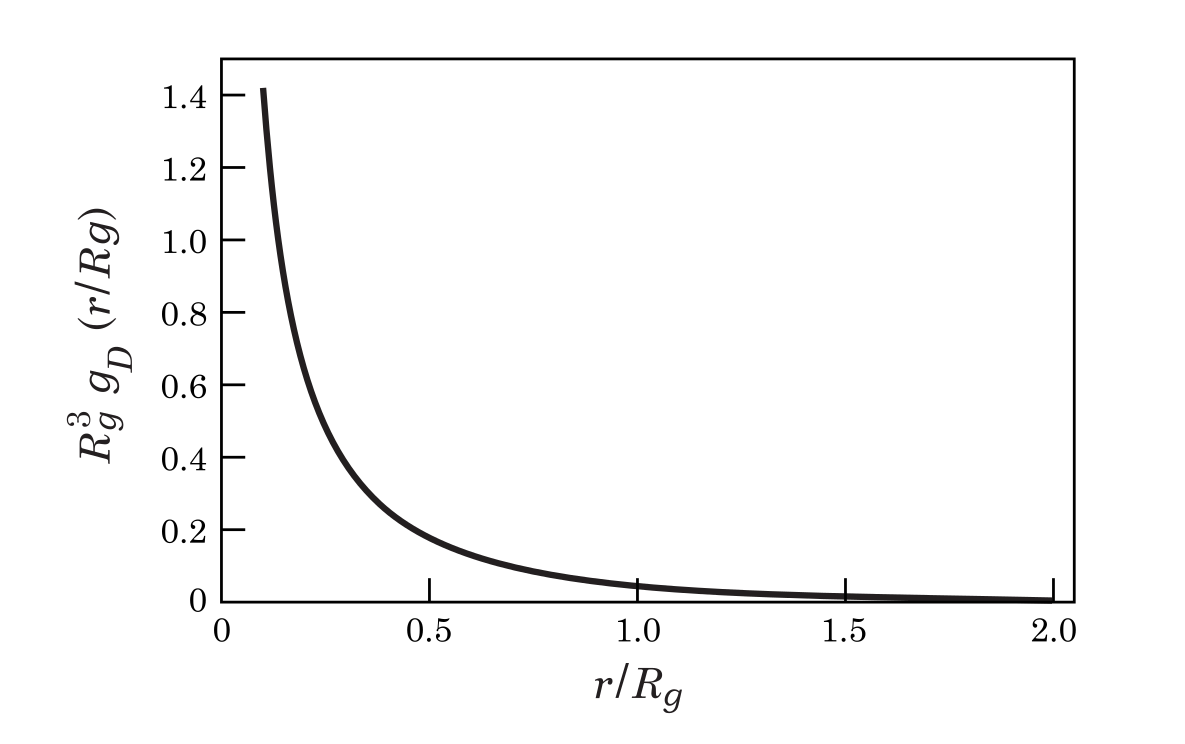
\includegraphics[scale=0.4]{Contents/chapter3/figures/FIG3-9.png}
	\caption{由(\ref{3.113})定义的Debye函数逆傅里叶变换,并以$\frac{r}{R_g}$为横坐标,以${R_g}^3 g_D(r)$为纵坐标.}
	\label{FIG3.9}
\end{figure}

形如(\ref{FIG3.9}),$\frac{r}{R_g} \ll 1$时,函数以$\frac{1}{r}$的速度代数衰减:
\begin{equation}
g_D(r) \sim \frac{3}{\pi b^2 N r}
\end{equation}
$r \sim R_g$时,函数单调的指数级的衰减为零:
$$g_D(r) \sim \frac{1}{r} e^{-\frac{\sqrt{3}r}{R_g}}$$

将弱非均匀性展开应用到其他聚合物体系(包括支链聚合物,共聚物)是非常直接的.

例如,在三臂星形均聚物的情况下,臂长相等,即$N_j = N$,
则
\begin{equation}
Q[w] = \frac{1}{V} \int [q(\br ,N;[w])]^3\,\mathrm{d} \br 
\end{equation}
又由(\ref{3.116})和(\ref{3.119})可得
\begin{equation}
Q[w] \sim e^{-3w_0 N} [1+\frac{3 {\epsilon_a}^2 N^2}{2V^2} \sum_{\mathbf{k}} \hat{g_S}(k^2 {R_g}^2)\hat{\omega}(\mathbf{k})\hat{\omega}(-\mathbf{k})+\dots]
\end{equation}
其中${R_g}^2 = \frac{Nb^2}{6}$为星形中一臂的旋转半径,$g_S(x)$为类Debye函数
\begin{equation}
\hat{g_S}(x) = \hat{g_D}(x) + 2[\hat{h_D}(x)]^2
\end{equation}
其中
\begin{equation}
\hat{h_D}(x) = \frac{1}{x} [1-e^{-x}]
\end{equation}
从而密度算子和对相关函数分别为
\begin{equation}
\rho(\br ;[w]) \sim \rho_0[1-\epsilon_a N \int g_S(|\br -\br ') \omega(\br ')\,\mathrm{d} \br '+O({\epsilon_a}^2)]
\end{equation}




\cite{tam19912d}
\bibliography{../ref}
\end{document}
